\documentclass[10pt,a4paper]{article}
\usepackage[utf8]{inputenc}
\usepackage{amsthm, amsmath, mathtools, amssymb}
\usepackage[left=2.3cm,right=2.3cm,top=3cm,bottom=3cm]{geometry}
\usepackage[colorlinks,linkcolor=blue,citecolor=blue,urlcolor=blue]{hyperref}
\usepackage{standalone}
\usepackage[catalan]{babel}
\usepackage{titlesec}
\usepackage{enumitem}
\usepackage{physics}
\usepackage[hypcap=false]{caption}
\titleformat{\section}
  {\normalfont\fontsize{11}{15}\bfseries}{\thesection}{1em}{}

\newcommand{\RR}{\ensuremath{\mathbb{R}}}
\newcommand{\QQ}{\ensuremath{\mathbb{Q}}}
\newcommand{\ZZ}{\ensuremath{\mathbb{Z}}}

\newcommand{\ii}{\mathrm{i}} % imaginary unit

\DeclareDocumentCommand\partialderivative{ s o m g d() }{ 
          % Total derivative
          % s: star for \flatfrac flat derivative
          % o: optional n for nth derivative
          % m: mandatory (x in df/dx)
          % g: optional (f in df/dx)
          % d: long-form d/dx(...)
            \IfBooleanTF{#1}
            {\let\fractype\flatfrac}
            {\let\fractype\frac}
            \IfNoValueTF{#4}
            {
                \IfNoValueTF{#5}
                {\fractype{\partial \IfNoValueTF{#2}{}{^{#2}}}{\partial #3\IfNoValueTF{#2}{}{^{#2}}}}
                {\fractype{\partial \IfNoValueTF{#2}{}{^{#2}}}{\partial #3\IfNoValueTF{#2}{}{^{#2}}} \argopen(#5\argclose)}
            }
            {\fractype{\partial \IfNoValueTF{#2}{}{^{#2}} #3}{\partial #4\IfNoValueTF{#2}{}{^{#2}}}\IfValueT{#5}{(#5)}}
        } % partial differential operator

\renewcommand{\theenumi}{\textbf{\arabic{enumi}}}
\renewcommand{\theenumii}{\textbf{\alph{enumii}}}
\renewcommand{\theenumiii}{\textbf{\roman{enumiii}}}

\renewcommand{\exp}[1]{\mathrm{e}^{#1}} % exponential function
\DeclareMathOperator*{\im}{Im}


\newtheorem{thm}{Teorema}
\newcommand{\R}{\mathbb R}
\newcommand{\RA}{\Rightarrow}
\newcommand{\ra}{\rightarrow}
\newcommand{\RL}{\Leftrightarrow}

\title{\bfseries\Large Seminari 1}

\author{Víctor Ballester, NIU: 1570866\\ Arturo Castaño, NIU: 1566489\\ Enric Garriga, NIU: 1565357}
\date{\parbox{\linewidth}{\centering
  Equacions diferencials II\endgraf
  Grau en Matemàtiques\endgraf
  Universitat Autònoma de Barcelona\endgraf
  Març de 2022}}

\setlength{\parindent}{0pt}
\begin{document}
\selectlanguage{catalan}
\maketitle
\section*{Problema 1}
Considerem el següent sistema diferencial:
\begin{equation}
  \begin{cases}
    \dot{x}=x(x-2)=P(x,y) \\
    \dot{y}=y(y-1)=Q(x,y)
  \end{cases}
\end{equation}
Comencem dibuixant el seu retrat de fase.
\subsubsection*{Apartat \emph{a})}
Busquem primer les rectes invariants del sistema. Prenem el polinomi $f(x,y)=ax+by+c=0$. Com que els polinomis $P(x,y)$ i $Q(x,y)$ tenen grau 2, deduïm que el cofactor de $f$ té 1 com a grau màxim. Denotem per $k(x,y)=k_1x+k_2y+k_3$ el cofactor de $f$. Per tant busquem:
$$\frac{\partial f}{\partial x}P+\frac{\partial f}{\partial y}Q=ax^2-2ax+by^2-by=kf=k_1ax^2+(k_3a+ck_1)x+bk_2y^2+(bk_3+ck_2)y+(ak_2+bk_1)xy+ck_3$$
Per resoldre això cal igualar els coeficients corresponents. D'entrada obtenim $a=k_1a$ (pel coeficient de $x^2$) i $b=k_2b$ (pel coeficient de $y^2$).
\begin{itemize}
  \item Si $a=0$, aleshores $ck_1=-2a=0$ (pel coeficient de $x$). També sabem que $ck_3=0$ i $bk_1=0$ (ja que no hi pot haver cap terme independent ni cap terme amb $xy$). Amb aquestes últimes equacions, si $b=0$, aleshores $c=0$ perquè s'ha de complir necessàriament que $f=0$. Però això no és cap recta. Per tant $b\neq 0$ i aleshores $k_2=1$ i, per tant, $bk_3+c=-b$ (pel coeficient de $y$) que és equivalent a $b(k_3+1)+c=0$. A l'equació $ck_3=0$, si $c=0$, llavors tenim $by=0$. És a dir, que l'eix de les $x$ és una recta invariant. En canvi, si $k_3=0$, aleshores $b=-c$ i per tant $by-b=0$, és a dir, $y=1$. És a dir, la recta $y=1$ també és invariant.
  \item Si $a\ne 0$, de la mateixa forma considerant $b=0$ s'acaba trobant que les rectes $x=0$ i $x=2$ també són invariants.
  \item Finalment, si es considera $a\neq 0$ i $b\neq 0$, aleshores tenim que $k_1=k_2=1$. Com el terme $xy$ ha de tenir coeficient nul, deduïm llavors que $a=-b$. Però combinant aquesta igualtat amb les equacions $ak_3+c=-2a$, $bk_3+c=-b$ i $ck_3=0$, obtenim un sistema que té com a única solució $a=b=c=0$, que no pot ser.
\end{itemize}
Per tant, únicament tenim les quatres rectes invariants següents: $x=0$, $y=0$, $x=2$ i $y=1$.
% Busquem primer les rectes invariants del sistema. Prenem el polinomi $f(x,y)=ax+by+c=0$. Com que els polinomis $P(x,y)$ i $Q(x,y)$ tenen grau 2, deduïm que el cofactor de $f$ té 1 com a grau màxim. Denotem per $k(x,y)=k_1x+k_2y+k_3$ el cofactor de $f$. Per tant busquem:
% $$\frac{\partial f}{\partial x}P+\frac{\partial f}{\partial y}Q=ax^2-2ax+by^2-by=kf=k_1ax^2+(k_3a+ck_1)x+bk_2y^2+(bk_3+ck_2)y+(ak_2+bk_1)xy+ck_3$$
% Per resoldre això cal igualar els coeficients corresponents: en un primer moment obtenim $a=k_1a$ i $b=k_2b$. Si $a=0 \implies ck_1=-2a=0$. També sabem que $ck_3=0$ i $bk_1=0$ (doncs no hi pot haver cap terme independent ni cap terme amb $xy$). En aquestes últimes equacions, si $b=0 \implies c=0$ doncs no oblidem que volem $f=0$. Però això no és cap recta. Per tant $b\neq 0 \implies k_2=1 \implies bk_3+c=-b \Leftrightarrow b(k_3+1)+9c=0$. A l'equació $ck_3=0$, si $c=0$, llavors tenim $by=0 \implies y=0$. És a dir, que l'eix de les $x$ és una recta invariant. En canvi, si $k_3=0 \implies b=-c \implies by-b=0 \Leftrightarrow y=1$. És a dir, la recta $y=1$ també és invariant.
% \par
% De la mateixa forma, si considerem $b=0$ s'acaba trobant que les rectes $x=0$ i $x=2$ també són invariants. Finalment, si es considera $a\neq 0$ i $b\neq 0 \implies k_1=k_2=1$. Com el terme $xy$ ha de tenir coeficient nul, deduïm llavors que $a=-b$. Però combinant aquesta igualtat amb les equacions $ak_3+c=-2a$, $bk_3+c=-b$ i $ck_3=0$, obtenim un sistema que té com a única solució $a=b=c=0$.
% \\
% Per tant, únicament tenim les quatres rectes invariants següents: $x=0$, $y=0$, $x=2$ i $y=1$.

\par
Fixem-nos ara que, si considerem $y=0$ o $y=1$ (i per tant $\dot{y}=0$), es tindrà que $\dot{x}>0$ si $x<0$ o $x>2$, i $\dot{x}<0$ si $0<x<2$. De la mateixa forma, si es considera $x=0$ o $x=2$ (i per tant $\dot{x}=0$), quan $y<0$ o $y>1$ s'obté que $\dot{y}>0$, mentre que $0<y<1 \implies \dot{y}<0$.
\\ Amb això deduïm que els punts $(0, 1)$ i $(2, 0)$ són selles, el punt $(0,0)$ és atractor i que el punt $(2,1)$ és repulsor. Aquest resultat es pot comprobar també amb el teorema de Hartman. Amb tot això ja podem deduir el retrat de fase del nostre sistema.

\begin{center}
  \begin{minipage}{\linewidth}
    \centering
    \includestandalone[mode=image|tex,width=0.7\linewidth]{Images/retrat1}
    \captionof{figure}{Retrat de fase del sistema diferencial}
  \end{minipage}
\end{center}

\subsubsection*{Apartat \emph{b})}
Tenint ja el retrat de fase deduït, ens demanem quins son els intervals maximals de definició de les solucions en funció de les condicions inicials. És a dir, busquem donar tota la informació possible sobre els intervals maximals de definició. Per això, utilitzarem el següent resultat:

\begin{thm}
  Considerem el següent sistema diferencial: \begin{equation}
    \begin{cases}
      \dot{x}=P(x,y) \\
      \dot{y}=Q(x,y)
    \end{cases}
  \end{equation}
  amb domini de definició $\Omega$. Sigui $I_p=(\alpha, \omega)$, amb $-\infty\leq \alpha <0< \omega\leq +\infty$, l'interval màxim de definició de la solució $\varphi_p(t)$ que verifica la condició inicial $\varphi_p(0)=p$.
  \\
  Llavors: \begin{itemize}
    \item	si $\omega<+\infty$, llavors $\varphi_p(t)$ \text{tendeix a la frontera de} $\Omega, \partial \Omega$, \text{quan t tendeix a} $\omega$.
    \item si $\alpha>-\infty$, llavors $\varphi_p(t)$ \text{tendeix a la frontera de} $\Omega, \partial \Omega$, \text{quan t tendeix a} $\alpha$.
  \end{itemize}
\end{thm}

En el nostre sistema, el domini de definició del sistema és $\R^2$, i per tant la seva frontera és \textquotedblleft l'infinit\textquotedblright (és a dir, que el domini de definició del sistema no està acotat). Per tant, a partir d'aquí ja podem assegurar que qualsevol solució que tingui com a condició inicial un punt $p=(x,y)$ tal que $0<x<2$ i $0<y<1$ té com a interval de definició $\R$ ja que quan $t$ decreix l'òrbita tendeix al punt $(2,1)$, mentre que quan $t$ creix l'òrbita tendeix a l'origen. Però cap d'aquests punts pertany a la frontera de $\R^2$. Per tant, pel recíproc del teorema deduïm que $I_p=\R$.
\\
De manera similar, a partir del recíproc del teorema, deduïm que, donat $p=(x,y)$:
\begin{itemize}
  \item si $x<0$ i $y<1$, aleshores l'interval de definició és $I_p=(\alpha, +\infty)$
  \item si $0<x<2$ i $y<0$, aleshores l'interval de definició és $I_p=(\alpha, +\infty)$
  \item si $0<x<2$ i $y>1$, aleshores l'interval de definició és $I_p=(-\infty, \omega)$
  \item si $x>0$ i $y>1$, aleshores $I_p=(-\infty, \omega)$
  \item si $x>2$ i $0<y<1$, aleshores $I_p=(-\infty, \omega)$
  \item si $x<0$ i $y>1$, aleshores no podem deduir res més: $I_p=(\alpha, \omega)$
  \item si $x>2$ i $y<0$, tampoc podem deduir res més: $I_p=(\alpha, \omega)$
\end{itemize}

En el cas de les rectes invariants tenim:
\begin{itemize}
  \item Per $x=0$ o per $x=2$:
        \begin{itemize}
          \item per $y<0$: $I_p=(\alpha, +\infty)$
          \item per $0<y<1$: $I_p=\R$
          \item per $y>1$: $I_p=(-\infty, \omega)$
        \end{itemize}
  \item Per $y=0$ o per $y=1$:
        \begin{itemize}
          \item per $x<0$: $I_p=(\alpha, +\infty)$
          \item per $0<x<2$: $I_p=\R$
          \item per $x>2$: $I_p=(-\infty, \omega)$
        \end{itemize}
\end{itemize}

Finalment, encara que no siguin punts de la frontera, és clar que les òrbites corresponents als punts d'equilibri tenen $\R$ com a domini de definició.

\subsubsection*{Extra}
Resolent el sistema diferencial de forma analítica es pot deduir l'interval de definició per qualsevol condició inicial. És a dir, calcular de manera explicita els intervals de solució. Fixem-nos que el sistema diferencial està format per equacions diferencials autònomes de la forma
\begin{equation}\label{3}
  \dv{\eta}{t}=\eta(\eta-a), \ \ a\in \R
\end{equation}

Aleshores el que farem serà resoldre l'equació \eqref{3} donada una condició inicial i deduir els intervals de definició.
\par
És clar que si considerem $\eta_0=0, a$, amb $\eta_0$ la condició inicial, llavors la solució és constantment $\eta_0$. Per tant, prenem $\eta_0\neq 0, a$. Aleshores, per el mètode de separació de variables, \eqref{3} es pot reescriure com:
\begin{equation}
  \frac{\dd{\eta}}{\eta(\eta-a)}=\left(\frac{1}{a(\eta-a)}-\frac{1}{a\eta}\right)\dd{\eta}=\dd{t}
\end{equation}
Integrant tenint en compte la condició inicial obtenim:
\begin{equation}
  t=\frac{1}{a}\left(\int_{\eta_0}^{\eta}\frac{\dd{x}}{x-a}-\int_{\eta_0}^{\eta}\frac{\dd{x}}{x}\right)\iff at=\left[\ln(x-a)\right]_{\eta_0}^\eta-\left[\ln(x)\right]_{\eta_0}^\eta=\ln\left(\frac{\eta-a}{\eta_0-a}\right)-\ln\left(\frac{\eta}{\eta_0}\right)
\end{equation}
Per continuar notem que cal que els elements que hi han dins dels logaritmes tinguin signe positiu. Per tant deduïm que (a partir d'ara suposarem $a>0$ per simplicitat):
\begin{itemize}
  \item Si $\eta_0<0$, aleshores $\eta<0$
  \item Si $0<\eta_0<a$, aleshores $0<\eta<a$
  \item Si $\eta_0>a$, aleshores $\eta>a$
\end{itemize}
Aleshores manipulant l'expressió obtenim:
\begin{equation*}
  at=\ln\left(\frac{\eta_0(\eta-a)}{\eta(\eta_0-a)}\right) \implies \eta(\eta_0-a)\exp{at}=\eta_0\eta-a\eta_0 \implies \eta[(\eta_0-a)\exp{at}-\eta_0]=-a\eta_0\implies \eta=\frac{a\eta_0}{\eta_0+(a-\eta_0)\exp{at}}
\end{equation*}
D'aquí podem deduir els intervals de definició de les solucions:

$$\eta_0+(a-\eta_0)\exp{at_0}=0 \iff \eta_0=(\eta_0-a)\exp{at_0} \iff t_0=\frac{1}{a}\ln\left(\frac{\eta_0}{\eta_0-a}\right)$$
Per trobar el límit per $t$ cal considerar diversos escenaris:
\begin{itemize}
  \item Si $\eta_0<0$, aleshores $\eta_0-a<\eta_0<0$ el que implica $0<\frac{\eta_0}{\eta_0-a}<1$ i per tant $t_0<0$. En aquest cas deduïm que l'interval de definició màxim serà $I=(t_0, +\infty)$
  \item Si $\eta_0>a$, aleshores $0<\eta_0-a<\eta_0$ el que implica $1<\frac{\eta_0}{\eta_0-a}$ i per tant $t_0>0$.
        En aquest cas deduïm que l'interval de definició màxim serà $I=(-\infty, t_0)$
  \item Si $0<\eta_0<a$, aleshores $\frac{\eta_0}{\eta_0-a}<0$ i per tant $t_0$ no està ben definit.
        En aquest cas deduïm que l'interval de definició màxim serà $I=(-\infty, +\infty)=\R$
\end{itemize}

Amb aquest cas estudiat podem donar tots els intervals de definició del sistema diferencial donat per l'enunciat per les diferents condicions inicials. Cal tenir en compte que, per l'interval $(\alpha, \omega)$, el valor de $\omega$ serà el mínim entre els $t_0$ de la solució per $x$ i $y$. De forma anàloga, $\alpha$ serà el màxim entre els dos valors de $t_0$ de les dues variables.
\begin{itemize}
  \item si $x<0$ i $y<0$, aleshores l'interval de definició és $I_p=(\alpha, +\infty)$ on $\alpha=\max\{\frac{1}{2}\ln\left(\frac{x_0}{x_0-2}\right), \ln\left(\frac{y_0}{y_0-1}\right)\}$
  \item si $x<0$ i $0<y<1$, aleshores l'interval de definició és $I_p=(\alpha, +\infty)$ on $\alpha=\frac{1}{2}\ln\left(\frac{x_0}{x_0-2}\right)$
  \item si $0<x<2$ i $y<0$, aleshores l'interval de definició és $I_p=(\alpha, +\infty)$ on $\alpha=\ln\left(\frac{y_0}{y_0-1}\right)$
  \item si $0<x<2$ i $y>1$, aleshores l'interval de definició és $I_p=(-\infty, \omega)$ on
        $\omega=\ln\left(\frac{y_0}{y_0-1}\right)$
  \item si $x>0$ i $y>1$, aleshores $I_p=(-\infty, \omega)$ on $\omega=\min\{\frac{1}{2}\ln\left(\frac{x_0}{x_0-2}\right), \ln\left(\frac{y_0}{y_0-1}\right)\}$
  \item si $x>2$ i $0<y<1$, aleshores $I_p=(-\infty, \omega)$ on
        $\omega=\frac{1}{2}\ln\left(\frac{x_0}{x_0-2}\right)$
  \item si $x<0$ i $y>1$, aleshores $I_p=(\alpha, \omega)$ on $\alpha=\frac{1}{2}\ln\left(\frac{x_0}{x_0-2}\right)$ i $\omega=\ln\left(\frac{y_0}{y_0-1}\right)$
  \item si $x>2$ i $y<0$, aleshores $I_p=(\alpha, \omega)$ on $\alpha=\ln\left(\frac{y_0}{y_0-1}\right)$ i $\omega=\frac{1}{2}\ln\left(\frac{x_0}{x_0-2}\right)$
\end{itemize}

En el cas de les rectes invariants:
\begin{itemize}
  \item Per $x=0$ o per $x=2$:
        \begin{itemize}
          \item per $y<0$: $I_p=(\alpha, +\infty)$ on $\alpha=\ln\left(\frac{y_0}{y_0-1}\right)$
          \item per $y>1$: $I_p=(-\infty, \omega)$ on $\omega=\ln\left(\frac{y_0}{y_0-1}\right)$
        \end{itemize}
  \item Per $y=0$ o per $y=1$:
        \begin{itemize}
          \item per $x<0$: $I_p=(\alpha, +\infty)$ on $\alpha=\frac{1}{2}\ln\left(\frac{x_0}{x_0-2}\right)$
          \item per $x>2$: $I_p=(-\infty, \omega)$ on $\omega=\frac{1}{2}\ln\left(\frac{x_0}{x_0-2}\right)$
        \end{itemize}
\end{itemize}

La resta de casos ja han estat obtinguts anteriorment.
\newpage
\section*{Problema 2}
Considerem el sistema diferencial
\begin{equation}\label{sistex2}
  \left\lbrace \begin{aligned}
     & \dot{x}=-y    \\
     & \dot{y}=x-x^2
  \end{aligned}\right.
\end{equation}
\subsubsection*{Apartat \emph{i})}
Sabem que és un sistema Hamiltonià. Per definició, això vol dir que existeix una funció $H(x,y)$ tal que $\displaystyle \dot{x}=-\frac{\partial H}{\partial y} \text{ i }\dot{y}=\frac{\partial H}{\partial x}$. Per tant en aquest cas tenim:
$$\left\lbrace \begin{aligned}
    -\frac{\partial H}{\partial y} & =-y    \\
    \frac{\partial H}{\partial x}  & =x-x^2
  \end{aligned}\right.\implies\left\lbrace \begin{aligned}
     & H=\frac{y^2}{2}+\phi(x)                  \\\
     & H=\frac{x^2}{2}-\frac{x^3}{3}+\varphi(y)
  \end{aligned}\right.\implies \boxed{H(x,y)=\frac{y^2}{2}+\frac{x^2}{2}-\frac{x^3}{3}}$$
És la integral primera del sistema.
\subsubsection*{Apartat \emph{ii})}
Ara, per dibuixar el retrat de fase comencem trobant els punts crítics, que sabem que són aquells que compleixen $(\dot{x},\dot{y})=(0,0)$.\\
Punts d'equilibri:
$$
  \left\lbrace \begin{aligned}
    \dot{x} & =0 \\
    \dot{y} & =0
  \end{aligned}\right.\implies
  \left\lbrace \begin{aligned}
    -y     & =0 \\
    x(1-x) & =0
  \end{aligned}\right.\implies
  \left\lbrace \begin{aligned}
    y & =0            \\
    x & =0\text{ o }1
  \end{aligned}\right.
$$
Aquest estudi ràpid ha revel·lat que el conjunt de punts crítics és $\{(0,0);(1,0)\}$.
\\Acabar de trobar la resta d'òrbites és fàcil ja que sabem que aquestes es troben a les corbes de nivell de la integral primera $H$. Per tant, tan sols hem de fer el retrat de les corbes $H(x,y)=h$, és a dir:
\begin{equation}
  \frac{y^2}{2}+\frac{x^2}{2}-\frac{x^3}{3}=h\quad\Longleftrightarrow\quad
  y=\pm\sqrt{\frac{2}{3}x^3-x^2+2h}
\end{equation}
Així doncs, cal dur a terme l'estudi de la funció $g_h(x)=\frac{2}{3}x^3-x^2+2h$ pels diversos valors $h$. Com $\sqrt{x}$ és una funció monòtona i $y=\pm\sqrt{g_h(x)}\;$ si $g$ creix, $|y|$ també ho fa i $g_h(x)=0\implies y=0$. Aleshores, les òrbites del sistema són molt semblants a la gràfica de $g_h(x)$ quan $g_h(x)\geq0$, i tota la regió $y<0$ és la \textquotedblleft reflexió\textquotedblright del semiplà $y>0$.

Estudiem, doncs, com és la gràfica de $g_h(x)$ per cada valor d'$h$:

\pagebreak
\underline{$h=0$}:\hspace{5cm} $\displaystyle g_0(x)=\frac{2}{3}x^3-x^2$
\begin{center}
  \begin{minipage}{\textwidth}
    \centering
    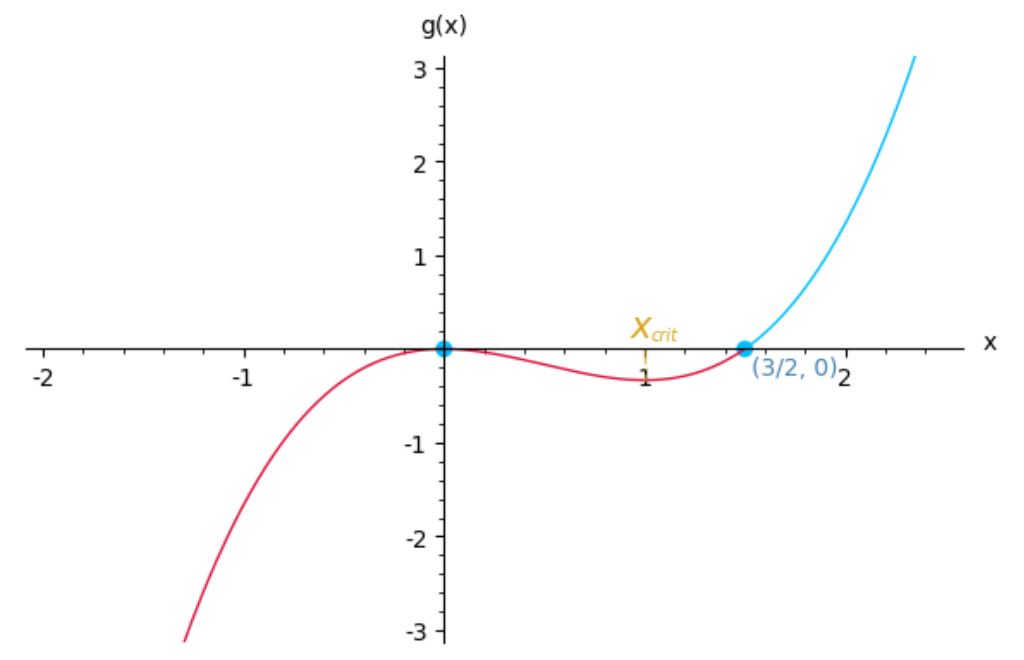
\includegraphics[scale=0.54]{Images/gh=0}
    \label{gh=0}
  \end{minipage}
\end{center}
Un estudi ràpid mostra que la funció $g_0$ és positiva per $x>3/2$. Això defineix una òrbita que talla l'eix $X$ a $x=3/2$, i va augmentant el valor de $y$ a mesura que $x$ creix. A més, també ens apareix el punt crític $(0,0)$. I recordem, un cop més, el retrat de fase també tindrà la reflexió respecte l'horitzontal de tots els resultats que anem trobant.
\\Per tant, de moment hem trobat dues òrbites (el punt crític més la branca de la dreta):
\begin{center}
  \begin{minipage}[h]{\textwidth}
    \centering
    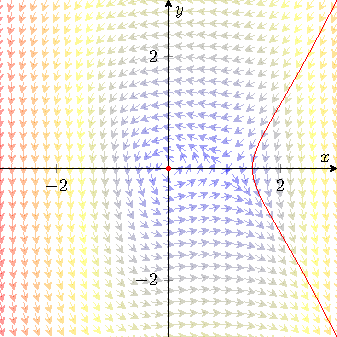
\includegraphics[scale=1.5]{Images/retrat2h0}
    %\caption{}
    \label{retrat0}
  \end{minipage}\vspace{2mm}
\end{center}

Notem que al retrat de fase hem inclòs les fletxes del camp vectorial per remarcar el sentit de recorregut de les òrbites. Aquestes fletxes les hem normalitzat, per a que no quedi tan atapeït, i en canvi hem introduït el codi de colors per denotar el seu mòdul (on blau significa mòdul petit fins a vermell, que significa un mòdul gran).

Ara, com que el paràmetre $h$ és només el terme independent de la funció $g_h(x)$, variar-lo no afectarà la curvatura de la funció, només la desplaçarà verticalment (cap a munt per $h>0$ i cap avall per $h<0$).

\pagebreak
\underline{$h<0$}:
\begin{center}
  \begin{minipage}[h]{\textwidth}
    \centering
    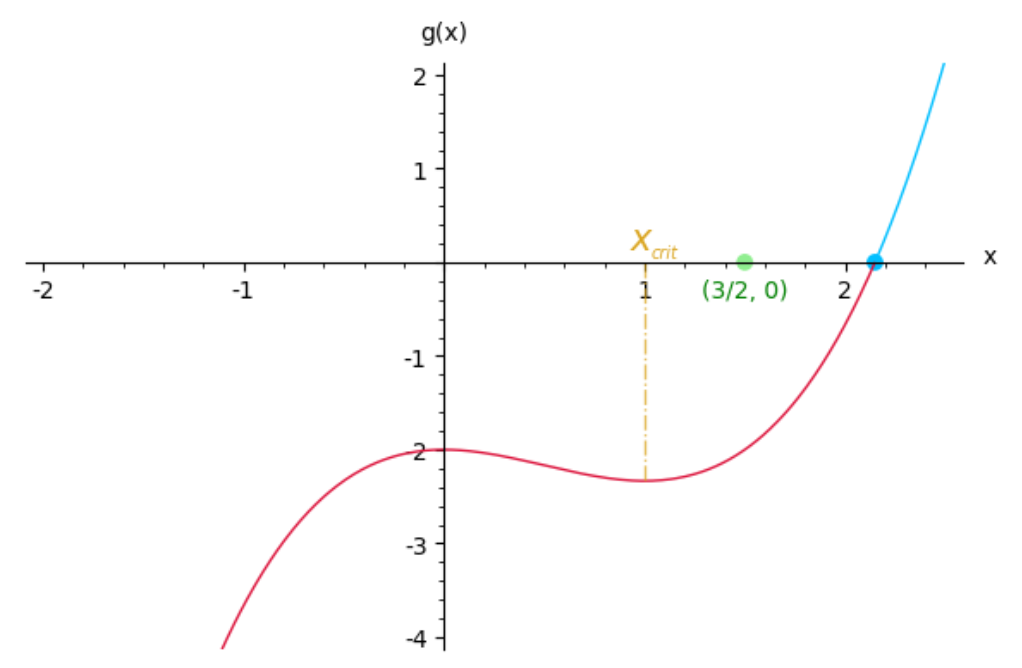
\includegraphics[scale=0.5]{Images/gh=-1}
    %\caption{}
    \label{gh=-1}
  \end{minipage}
\end{center}
Per tots els diversos valors d'$h<0$ possibles, les òrbites estan definides a partir d'una abscissa $x_0>3/2$ (punt blau) atès que $g_h>0$ només en aquella regió. Un cop més, augmentarà la $y$ a mesura que creixi la $x$. És a dir, els diversos valors d'$h<0$ generen tota una família d'òrbites similars a la branca definida per $h=0$, i que es trobaran a la dreta d'aquesta:
\begin{center}
  \begin{minipage}[h]{\textwidth}
    \centering
    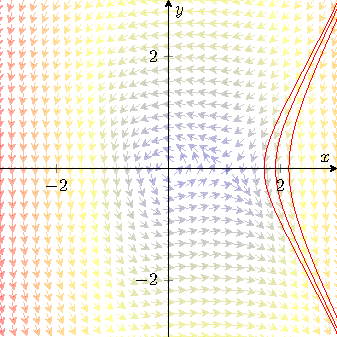
\includegraphics[scale=1.5]{Images/retrat2h-1}
    %\caption{}
    \label{retrat-1}
  \end{minipage}
\end{center}
Finalment, cal separar en 3 parts el cas $h>0$ ja que, com es pot veure intuïtivament a partir de les imatges, existeix un valor $a>0$ per al qual $g_a$ tindrà dues regions positives (per tant amb òrbites definides) tocant-se en un cert $x_{crit}$ (el mínim de $g_a$), on $g_a(x_{crit})=0$. Aleshores per	$0<h<a$ tindrem tres talls amb l'eix horitzontal mentres, per $h>a$, $g_h$ tindrà una sola arrel a partir de la qual tota una òrbita estarà definida.
\\Fent diversos càlculs per trobar el mínim relatiu de $g_h$ tot imposant $g'_h(x)=0$, veiem $x_{crit}=1$, i igualant $g_a(1)=0$ per aïllar la $a$, obtenim el valor $\boxed{a=1/6}$. Ara presentem-ho gràficament:

\pagebreak
\underline{$0<h<a$}:
\begin{center}
  \begin{minipage}[h]{0.57\textwidth}\hspace{3mm}
    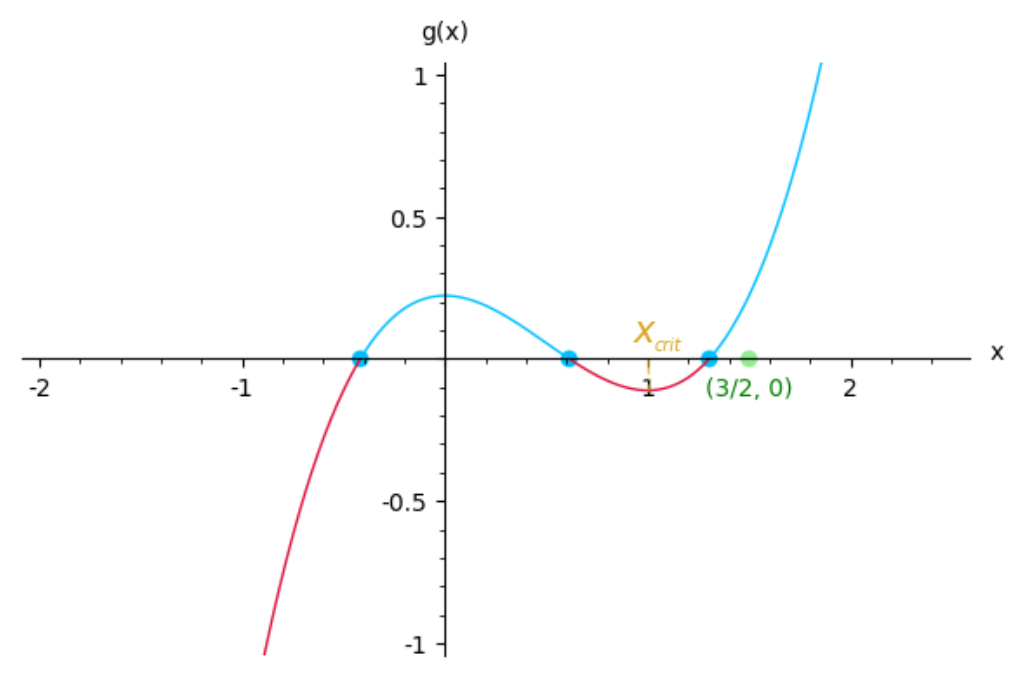
\includegraphics[scale=0.4]{Images/gh=1i9}
    %\caption{}
    \label{gh=1i9}
  \end{minipage}\hfill
  \begin{minipage}[h]{0.43\textwidth}
    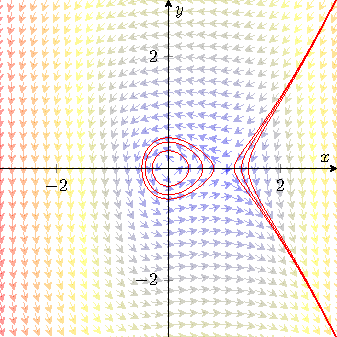
\includegraphics[scale=1.1]{Images/retrat2h1i9}
    %\caption{}
    \label{retrat1i9}
  \end{minipage}
\end{center}
\underline{$h=a=\frac{1}{6}$}:
\begin{center}
  \begin{minipage}[c]{0.57\textwidth}\hspace{3mm}
    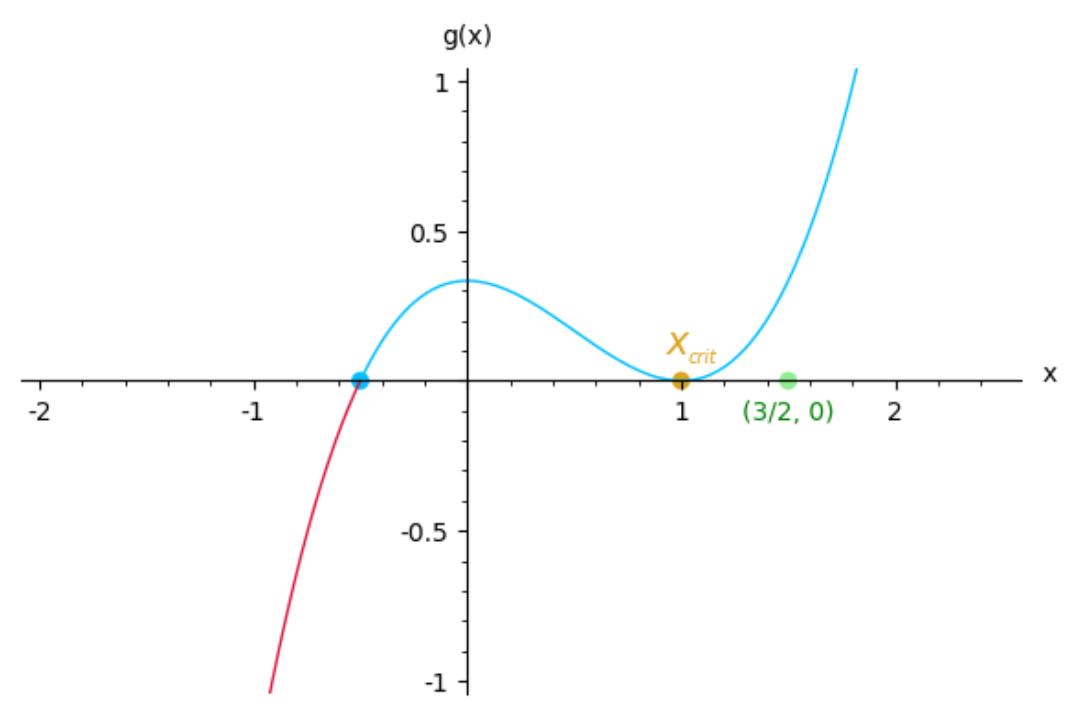
\includegraphics[scale=0.38]{Images/gh=a}
    %\caption{}
    \label{gh=a}
  \end{minipage}\hfill
  \begin{minipage}[h]{0.43\textwidth}
    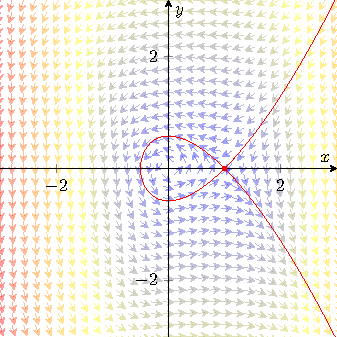
\includegraphics[scale=1.1]{Images/retrat2h1i6}
    %\caption{}
    \label{retrat1i6}
  \end{minipage}
\end{center}

\underline{$h>a$}:
\begin{center}
  \begin{minipage}[h]{0.57\textwidth}\hspace{3mm}
    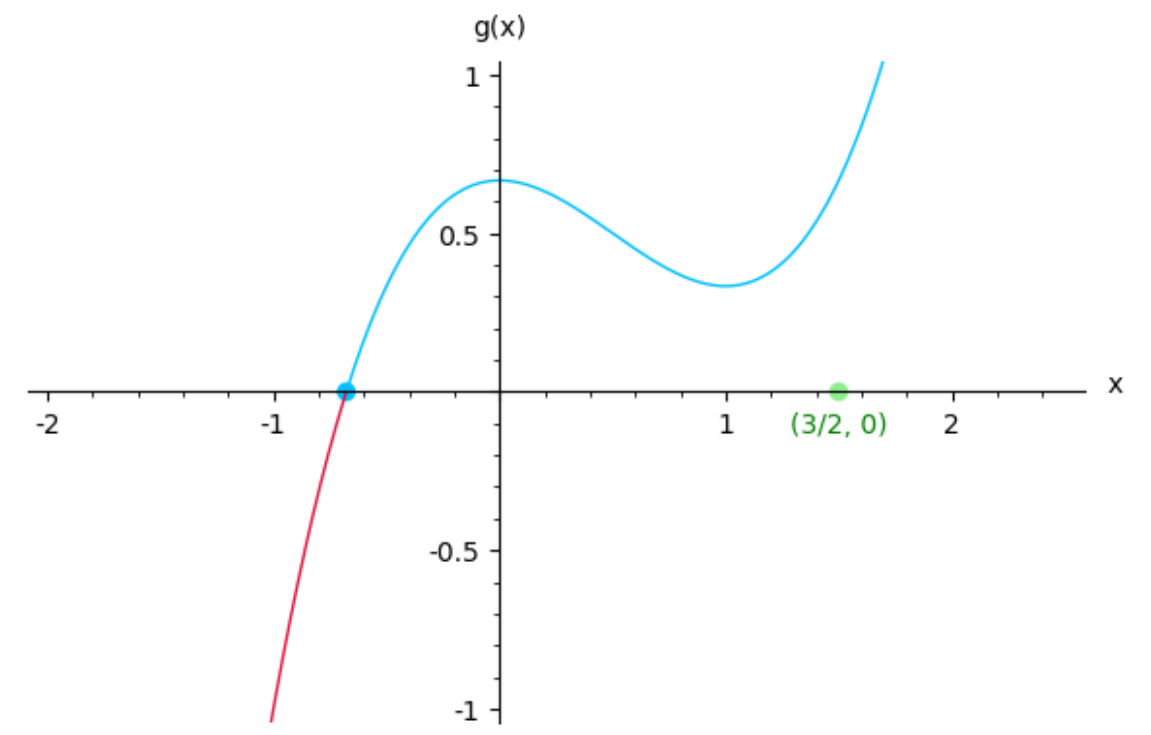
\includegraphics[scale=0.36]{Images/gh=2i6}
    %\caption{}
    \label{gh=2i6}
  \end{minipage}\hfill
  \begin{minipage}[h]{0.43\textwidth}
    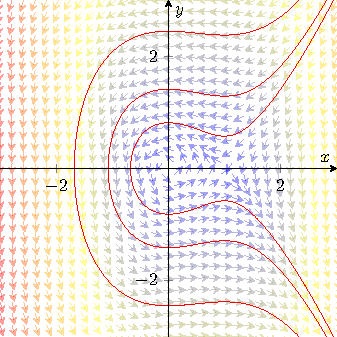
\includegraphics[scale=1.1]{Images/retrat2h2i6}
    %\caption{}
    \label{retrat2i6}
  \end{minipage}
\end{center}

Així, posant en comú tots els resultats obtinguts aconseguim el següent retrat de fase:
\begin{center}
  \begin{minipage}[h]{\textwidth}
    \centering
    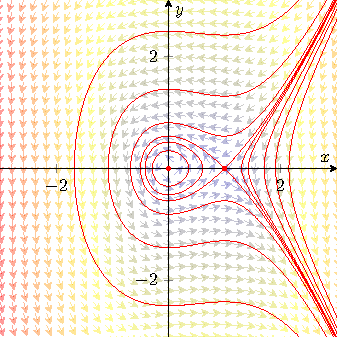
\includegraphics[scale=2]{Images/retrat2htot}
    %\caption{}
    \label{retrat2tot}
  \end{minipage}
\end{center}
\subsubsection*{Apartat \emph{iii})}
Clarament, els sistemes Hamiltonians poden tenir òrbites periòdiques. Per exemple, considerem el sistema
$$
  \left\lbrace
  \begin{aligned}
    x & =-y \\
    y & =x
  \end{aligned}
  \right.
$$
que té el Hamiltonià $\displaystyle H(x,y)=\frac{x^2+y^2}{2}$ i, justament, totes les òrbites d'aquest sistema són periòdiques (veure problema 3) atès que són tots els cercles del pla centrats a l'origen.
\subsubsection*{Apartat \emph{iv})}
En canvi, un sistema Hamiltonià no pot tenir cap cicle límit. Demostrem-ho per contradicció:

\begin{minipage}[h]{7cm}
  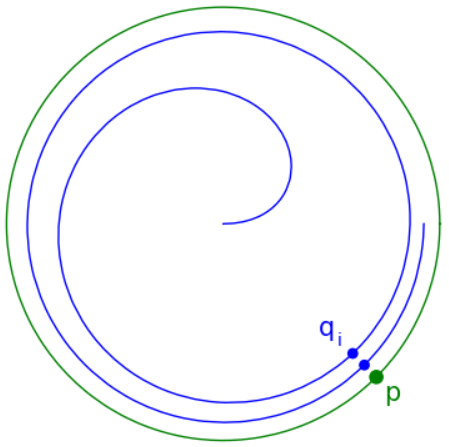
\includegraphics[scale=0.7]{Images/ciclim}
  %\caption{}
  \label{ciclim}
\end{minipage}\vspace{3mm}
\begin{minipage}[h]{8.2cm}
  Suposem que tenim un sistema diferencial Hamiltonià amb $H$ la seva integral primera. Considerem que aquest sistema té un cicle límit $\gamma$. El retrat de fase seria semblant al de la figura de l'esquerra (representació del cas dos-dimensional, però és valid per $2n$ dimensions), amb el cicle límit pintat de verd. Sigui $p\in\gamma$. Aleshores $H(p)=h$ per una certa $h$ constant. Ara volem provar que $\exists V$ un entorn de $p$ on $H|_V=h$, és a dir, on la integral primera és constant en tot l'entorn, el qual és una contradicció. Com $\gamma$ és cicle límit, $\exists V$ entorn de $p$ tal que $\forall q\in V$, l'orbita del punt ($\gamma_q$) s'apropa (ja sigui en temps positiu o negatiu, el cas és que hi ha punts de l'òrbita arbitràriament propers) al cicle límit $\gamma$.
\end{minipage}

Per tant, l'òrbita $\gamma_q$ conté una successió de punts $\{q,q_2,q_3,\dots,q_i\dots\}$ tal que $q_i\xrightarrow[]{i\to\infty}p$. És clar que, com $\gamma_q$ està continguda en una corba de nivell d'$H$, tenim $H(q_i)=c\enskip\forall i\in\mathbb{N}$.
\\I aquí ve el cop de gràcia. Que $H$ sigui integral primera vol dir que és diferenciable. En particular, contínua, i per tant $\displaystyle \lim_{x\rightarrow p}H(x)=H(p)$. En aquest cas,
$$
  \lim_{i\to\infty}H(q_i)=H(p)\iff \boxed{c=h}
$$
Per tant, en efecte $H(q)=h\enskip \forall q\in V$, demostrant així que $H$ és constant en un entorn de $p$ i arribant, finalment, a contradicció.
\\\qed
\newpage
\section*{Problema 3}
\subsubsection*{Sistema \texorpdfstring{$x''=-x$}{x''=-x} (osci\lgem ador harmònic)}
Observem primer de tot que el sistema $x''=-x$ és equivalent al sistema diferencial al pla següent:
\begin{equation}\label{sist1}
  \left\{
  \begin{aligned}
     & x' =y   \\
     & y'  =-x
  \end{aligned}
  \right.
\end{equation}
Aquest sistema només té un punt crític: l'origen. Vegem que $H_1(x,y)=x^2+y^2$ és una integral primera del sistema. En efecte, tenim que:
$$\pdv{H_1}{x}(x,y)\cdot y+\pdv{H_1}{y}(x,y)\cdot (-x)=(2x)y-(2y)x=0$$
Per tant, les òrbites del retrat de fase seran les solucions de les corbes de nivell $$H_1(x,y)=k\iff x^2+y^2=k\quad k\in\RR$$
Clarament aquestes corbes són cercles centrats a l'origen i cadascun de radi $\sqrt{k}$. Per determinar el sentit de gir de les òrbites, observem que quan partim de la condició inicial $(x_0,0)$, amb $x_0>0$, tenim que en un entorn d'aquest punt $y'<0$ i, per tant, l'òrbita girarà en sentit horari. Per continuïtat de les solucions respecte condicions inicials, totes les òrbites (que són periòdiques) giraran en sentit horari.
El retrat de fase del sistema diferencial \eqref{sist1} és el següent:
\begin{center}
  \begin{minipage}{\linewidth}
    \centering
    \includestandalone[mode=image|tex,width=0.8\linewidth]{Images/retrat31}
    \captionof{figure}{Retrat de fase del sistema $x''=-x$. Les corbes vermelles representen òrbites, quatre de les quals són periòdiques, i l'altra és un punt crític.}
  \end{minipage}
\end{center}
Notem que hem fet servir el mateix codi de colors per a les fletxes del camp vectorial que en l'exerici 2.

Deduïm doncs, que el punt crític es tracta d'un centre.
\subsubsection*{Sistema \texorpdfstring{$x''=-sin(x)$}{x''=-sin(x)} (pèndol simple)}

Observem primer de tot que el sistema $x''=-\sin x$ és equivalent al sistema diferencial al pla següent:
\begin{equation}\label{sist2}
  \left\{
  \begin{aligned}
     & x' =y        \\
     & y'  =-\sin x
  \end{aligned}
  \right.
\end{equation}
Calculem els punts crítics del sistema. Tenim que:
\begin{equation*}
  \left\{
  \begin{aligned}
    y       & =        0 \\
    -\sin x & =  0
  \end{aligned}
  \right.
  \iff x=\pi k, y=0\quad k\in\ZZ
\end{equation*}
És a dir, el sistema tindrà infinits punts crítics. Calculem ara una integral primera del sistema.
Per això cal buscar una funció $H_2(x,y)$ que satisfaci les equacions següents:
$$
  \left\{
  \begin{aligned}
    \pdv{H_2}{y}(x,y) & = -y     \\
    \pdv{H_2}{x}(x,y) & =-\sin x
  \end{aligned}\right.
  \implies
  \left\{
  \begin{aligned}
    H_2(x,y) & = -\frac{y^2}{2}+C_1(x) \\
    H_2(x,y) & =\cos x+C_2(y)
  \end{aligned}\right.
$$
Per tant, podem prendre la funció $H_2(x,y)=-\frac{y^2}{2}+\cos x$, que és una integral primera del sistema. Per tant, les òrbites del retrat de fase seran les solucions de les corbes de nivell: $$H_2(x,y)=h\iff -\frac{y^2}{2}+\cos x=h\iff y=\pm\sqrt{2}\sqrt{\cos x-h}\quad h\in\RR$$
Denotem per $f_h(x)=\cos x-h$ i estudiem el comportament d'aquest funció. D'entrada, observem que si $h\leq -1$, $f_h(x)\geq 0$ i si $h> 1$, $f_h(x)<0$. Per tant, una condició necessària perquè es compleixi que $f_h(x)\geq 0$ és que $h\in(-\infty,1]$. A més, donat un $h\in [-1,1]$ tindrem que: $$f_h(x)\geq 0\iff \cos x\geq h\iff x\in[2\pi n-\arccos h,2\pi n+\arccos h]\quad n\in\ZZ$$
D'aquest últim resultat i observant la periodicitat del $\sin x$ en \eqref{sist2} deduïm que el retrat de fase serà ``periòdic'' (de període $2\pi$) en l'eix $x$. Al gràfic següent es mostra la representació gràfica de $f_h(x)$ per alguns valors de $h$.
\begin{center}
  \begin{minipage}{\linewidth}
    \centering
    \includestandalone[mode=image|tex,width=0.7\linewidth]{Images/grafic2}
    \captionof{figure}{Gràfic de la funció $f_h(x)=\cos x-h$ per a diferents valors de $h$.}
  \end{minipage}
\end{center}
Observant la part positiva de la gràfica de $f_h(x)$ ja ens podem fer una idea de com serà el retrat de fase. Per determinar el sentit de gir de les òrbites, observem que quan partim de la condició inicial $(\pi/2,0)$ tenim que en un entorn d'aquest punt $y'<0$ i, per tant, en un entorn de $(\pi/2,0)$ la coordenada $y$ és decreixent. Per continuïtat de les solucions respecte condicions inicials, ja podem obtenir el sentit de totes les òrbites del sistema.
El retrat de fase del sistema diferencial \eqref{sist2} és, doncs, el següent:
\begin{center}
  \begin{minipage}{\linewidth}
    \centering
    \includestandalone[mode=image|tex,width=0.8\linewidth]{Images/retrat32}
    \captionof{figure}{Retrat de fase del sistema $x''=-\sin x$. Les corbes vermelles representen òrbites. En aquest cas tenim punts crítics, òrbites homeomorfes a $S^1$ i òrbites homeomorfes a $\RR$.}
  \end{minipage}
\end{center}

A posteriori i a causa de la simetria del retrat de fase deduïm que els punts crítics de la forma $2\pi k$, $k\in\ZZ$, són centres mentre que els punts de la forma $\pi(2k+1)$, $k\in\ZZ$, són selles.
\subsubsection*{Sistema \texorpdfstring{$x''=-1/x^2$}{x''=-1/x2} (camp gravitatori)}

Observem primer de tot que el sistema $x''=-1/x^2$ és equivalent al sistema diferencial al pla següent:
\begin{equation}\label{sist3}
  \left\{
  \begin{aligned}
     & x' =y               \\
     & y'  =-\frac{1}{x^2}
  \end{aligned}
  \right.
\end{equation}
Primer de tot cal remarcar que el domini de definició del sistema és, a diferència de tots els sistemes anteriors, $\RR^2\setminus\{x=0\}$.

D'altra banda, aquest sistema no té punts crítics perquè la segona equació no s'anul·la mai. Calculem ara una integral primera del sistema.
Per això cal buscar una funció $H_3(x,y)$ que satisfaci les equacions següents:
$$
  \left\{
  \begin{aligned}
    \pdv{H_3}{y}(x,y) & = -y            \\
    \pdv{H_3}{x}(x,y) & =-\frac{1}{x^2}
  \end{aligned}\right.
  \implies
  \left\{
  \begin{aligned}
    H_3(x,y) & = -\frac{y^2}{2}+C_1(x) \\
    H_3(x,y) & =\frac{1}{x}+C_2(y)
  \end{aligned}\right.
$$
Per tant, podem prendre la funció $H_3(x,y)=-\frac{y^2}{2}+\frac{1}{x}$, que és una integral primera del sistema. Per tant, les òrbites del retrat de fase seran les solucions de les corbes de nivell: $$H_3(x,y)=h\iff -\frac{y^2}{2}+\frac{1}{x}=h\iff y=\pm\sqrt{2}\sqrt{\frac{1}{x}-h}\quad h\in\RR$$
Denotem per $g_h(x)=\frac{1}{x}-h$ que està definida a $\RR^*$ i estudiem el comportament d'aquest funció. D'entrada, observem que $\displaystyle\lim_{x\to\pm\infty}g_h(x)=-h$, $\displaystyle\lim_{x\to 0^-}g_h(x)=-\infty$ i $\displaystyle\lim_{x\to 0^+}g_h(x)=+\infty$. A més, ${g_h}'(x)=-\frac{1}{x^2}<0\ \forall x\in\RR^*$. Per tant, la funció és sempre decreixent. Així doncs, ja tenim suficient informació per fer una representació gràfica de $g_h(x)$:
\begin{center}
  \begin{minipage}{\linewidth}
    \centering
    \includestandalone[mode=image|tex,width=0.7\linewidth]{Images/grafic3}
    \captionof{figure}{Gràfic de la funció $g_h(x)=\frac{1}{x}-h$ per a diferents valors de $h$.}
  \end{minipage}
\end{center}
Observant la part positiva de la gràfica de $g_h(x)$ ja ens podem fer una idea de com serà el retrat de fase. Per determinar el sentit de gir de les òrbites, observem que quan partim de la condició inicial $(x_0,0)$ tenim que en un entorn d'aquest punt $y'<0$ i, per tant, en un entorn de $(x_0,0)$ la coordenada $y$ és decreixent. Per continuïtat de les solucions respecte condicions inicials, ja podem obtenir el sentit de totes les òrbites del sistema.
El retrat de fase del sistema diferencial \eqref{sist3} és, doncs, el següent:
\begin{center}
  \begin{minipage}{\linewidth}
    \centering
    \includestandalone[mode=image|tex,width=0.8\linewidth]{Images/retrat33}
    \captionof{figure}{Retrat de fase del sistema $x''=-1/x^2$. Les corbes vermelles representen òrbites, totes elles homeomorfes a $\RR$.}
  \end{minipage}
\end{center}

\end{document}
